\documentclass[12pt,letterpaper]{scrartcl}
\usepackage{lipsum}
\usepackage[utf8]{inputenc}
\usepackage{amsmath}
\usepackage{amsfonts}
\usepackage{amssymb}
\usepackage{graphicx}
\usepackage[left=3cm,right=2.5cm,top=2.5cm,bottom=2.5cm]{geometry}
\usepackage[]{algorithm2e}
\author{Don cuyi}

%Color
\usepackage{color}
\definecolor{nred}{RGB}{174,49,54}
\definecolor{nblue}{RGB}{86,99,146}
\definecolor{nalgo}{RGB}{188,139,76}
\usepackage{sectsty}
\sectionfont{\color{nred}}
\subsectionfont{\color{nblue}}
\subsubsectionfont{\color{nalgo}}

%Librías tikz
\usepackage{pgf,tikz}
\usepackage{mathrsfs}
\usetikzlibrary{arrows}
\usetikzlibrary[patterns]
\newcommand{\degre}{\ensuremath{^\circ}}
\definecolor{qqwuqq}{rgb}{0.,0.39215686274509803,0.}
\definecolor{ffttww}{rgb}{1.,0.2,0.4}
%Hipervinculos
\usepackage{hyperref}

\usepackage{fancyhdr}
\pagestyle{fancy}
\fancyhead[L]{Combinaciones}
\fancyhead[C]{Licenciatura en ciencias de la computación}
\fancyhead[R]{USACH}

%interlineado
\renewcommand{\baselinestretch}{1.2}

%\bibitem{Yahoo} \textsc{Andres G} (2009),
%\textbf{¿Generar números aleatorios negativos en Lenguaje C?} En \textsc{Yahoo! respuestas}
%Recuperado el el 23 del julio del 2014
%\url{https://es.answers.yahoo.com/question/index?qid=20091121055249AAUQH3N}

\newcommand{\biblio}[7]{
\bibitem{#1} \textsc{#2} (#3),
\textbf{#4} En \textsc{#5}
Recuperado el #6
\url{#7}
}

% Last, F. M. (Year Published) Book. City, State: Publisher.
\newcommand{\book}[5]{
\bibitem{#1} \textsc{#2} (#3),
\textbf{#4}  \textsc{#5} Estado: Publicado
}

\begin{document}

\begin{titlepage}

\begin{center}

{\Large { Licenciatura en ciencia de la computación} }


\includegraphics[scale=1]{UDSCNRJ}
\\[1cm]

{\Huge \textsc{Combinaciones}}\\[0.7cm]

{\huge  Matemática Computacional}\\[2cm]


\begin{minipage}[l]{0.4\textwidth}
	\begin{flushleft}
	\linespread{1}
		\textbf{\textsf{Profesor:}}\\
		\large Nicolas Thériault
	\end{flushleft}
\end{minipage}
\begin{minipage}[l]{0.4\textwidth}

	\begin{flushright}

		\textbf{\textsf{Autor:}}\\
		\linespread{1}
		\large Sergio Salinas\\
		\large Danilo Abellá\\

	\end{flushright}
\end{minipage}

\end{center}

\end{titlepage}

\section*{Introducción}

En este informe se pretende mostrar las distintas formas y/o estrategias para calcular la combinatoria de n y r valores , para lo cual se utilizaron distintas técnicas y estrategias tanto algo-rítmicamente como en el uso de conocimiento matemático, además claro de formas de programación.

Cabe mencionar que se utilizó la librería gmp como forma de cálculo mas rápido, todo esto en lenguaje C/C++.

\newpage

\section{Algoritmo Implementado}

\section{Estrategía uno}

Esta estrategía es la más simple, solo se calcularon los valores n!, (n-r)! y r!, luego  se obtuvo la combinatoria multiplicando r! por (n-r)! y diviendo n! por el resultado de la multiplicación anterior.

\subsection{Estrategía dos}

Para la creación de este algoritmo se baso en el siguiente ejemplo:
\[\begin{matrix}
{7 \choose 4}  &= \dfrac{7!}{4! \cdot 3!} = \dfrac{7 \cdot 6 \cdot 5}{3 \cdot 2}\\ 
 &\\
{7 \choose 3}  &= \dfrac{7!}{3!\cdot4!} = \dfrac{7 \cdot 6 \cdot 5}{3 \cdot 2 }\\
\end{matrix}
\]

Gracias a la propiedad de simetría da el mismo resultado pero con los resultados cambiados, cuando $n-r > r$ ocurre que el mayor número del denominador se queda a la derecha en caso contrario el mayor se queda la izquierda.

Además se eso se observa cuando se factoriza factoriales el númerador queda de la forma $n \cdot (n-1) \cdot \ldots \cdot (r+1)!$, en base a todo esto se creo el siguiente algoritmo

\begin{itemize}
\item Se comprueba cuál número es más grande, si r ó n-r.


\item Se calcula la multiplicación de r + 1 o (n -r) + 1 (el que sea el mayor) hasta n, de esta forma se simula como si hubiera factorizado n a mayor denominador.

\item Se calcula el factorial del denominador menor.

\item Se calcula la combinatoria diviendo el numerador por el denominador.

\end{itemize}




\subsection{Estrategía tres}

Se aplico el mismo algoritmo que en la estrategía uno pero se cambiaron los mpz por mpf para así usar el punto flotante en los calculos.

\subsection{Estregía cuatro}


En este problema se utilizó la combinación numérica con la estrategia 2.2 mediante la cual sacamos el valor de una combinatoria utilizando el factorial de la división entre la variable n y r respectivamente , con r < n.

Para dicha estrategia se utilizó un algoritmo que primero saca el valor de la primera división ( en real ) , luego le resta 1 tanto al denominador como al numerador , y multiplica el resultado de la nueva división ( en real ) con el resultado de la primera… y así sucesivamente hasta que r = 1.

Una vez finalizado se tendría el valor de la combinatoria tras todas las multiplicaciones de cada fracción en cada ciclo recorrido.

\subsection{Estrategía cinco}

En este caso en nuestra fórmula de Striling el algoritmo se encarga de calcular primero el valor del numerador en la división de dicha fórmula, luego saca el exponencial elevado a n para tener el denominador , y una vez ambos sacados se divide y se multiplica por la raiz de 2*pi, este procedimiento se realiza primero con n, luego con r y finalmente con (n-r) para sacar sus respectivas aproximaciones de factoriales.  

Al final del algoritmo se divide la factorial de n por el producto entre r y ( n – r ).

\newpage

\section{Formulación experimentos}

Para probar los algoritmos se hizo un script en bash que compilara una vez y ejecutara varias veces el ejecutable, variando los metodos de entrada. 

A cada estrategía se le asigno un n fijo de 1000 y un r inicial de 1, el script va ejecuntando el algoritmo multiples veces haciendo creer a r hasta que alcanza n.


\newpage
\section{Información de Hardware y Software}


\subsection{ Notebook - Danilo Abellá}
\subsubsection{Software}
\begin{itemize}
\item SO: Xubuntu 16.04.1 LTS
\item GMP Library
\item Mousepad 0.4.0
\end{itemize}

\subsubsection{Hardware}
\begin{itemize}
\item AMD Turion(tm) X2 Dual-Core Mobile RM-72 2.10GHz
\item Memoria (RAM): 4,00 GB(3,75 GB utilizable)
\item Adaptador de pantalla: ATI Raedon HD 3200 Graphics
\end{itemize}




\subsection{Notebook - Sergio Salinas}
\subsubsection{Software}
\begin{itemize}
\item  SO: ubuntu Gnome 16.04 LTS
\item Compilador: gcc version 5.4.0 20160609 
\item Editor de text: Atom
\end{itemize}

\subsubsection{Hardware}
\begin{itemize}
\item Procesador: Intel Core i7-6500U CPU  2.50GHz x 4 
\item Video: Intel HD Graphics 520 (Skylake GT2) 
\end{itemize}


\newpage

\section{Curvas de desempeño de resultados}

\subsection{Estrategía uno}

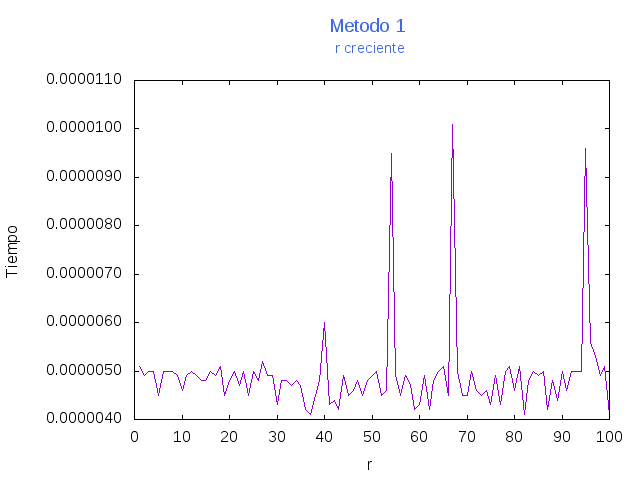
\includegraphics[scale=1]{Metodo1/plot1m1}

\subsection{Estrategia dos}

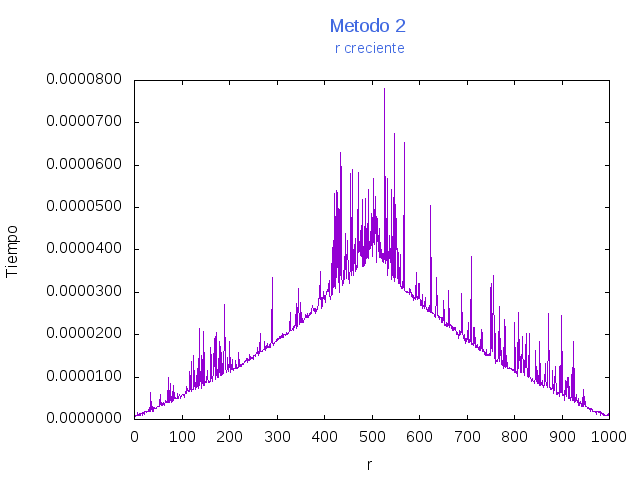
\includegraphics[scale=1]{Metodo2/plot1m2}

\subsection{Estrategia tres}

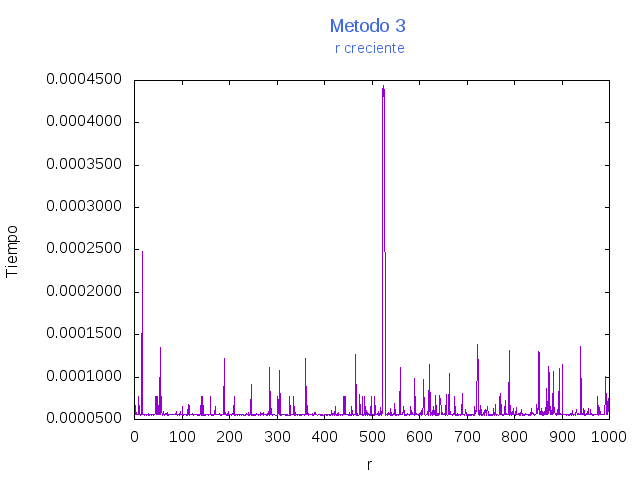
\includegraphics[scale=1]{Metodo3/plot1m3}

\subsection{Estrategia cuatro}

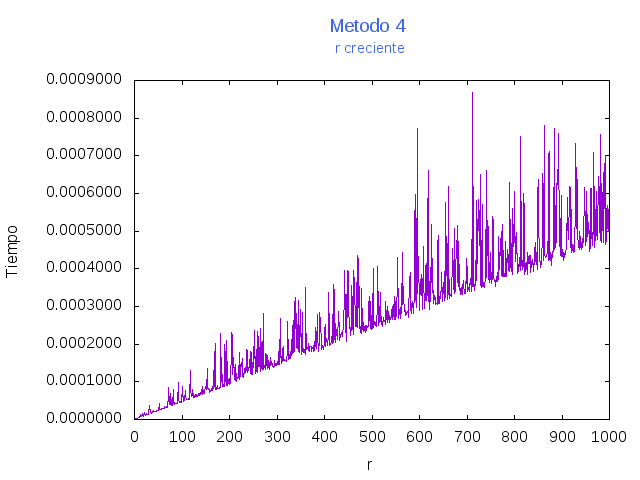
\includegraphics[scale=1]{Metodo4/plot1m4}

\subsection{Estretegia cinco}

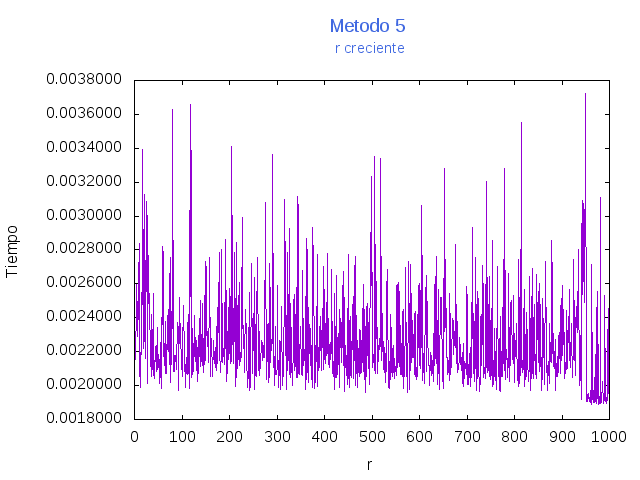
\includegraphics[scale=1]{Metodo5/plot1m5}

\newpage
\section{Conclusiones}

Gracias a los graficos se puede llegar a las sigueitnes conclusiones:

\begin{itemize}
\item La estrategia uno es eficiente cuando se trata de combinatorias en donde el n y r sean cercanos, pero aun así, fue la estrategia que tuva más costes de tiempo.
\item La estrategia dos es eficiente cuando se trata de combinatorias en donde el n y r sean lejanos entre si.
\item La estrategia tres tiene un coste superior a la estrategia dos pero el tiempo es parejo independiente de los valores de n y r.
\item La estrategia cuatro es eficiente para valores de r pequeños pero muy costosa para valores de r cercano al n, llegando a superar a la estrategia uno en lo que es el coste de tiempo.
\item La estrategia cinco es la menos eficiente y no parece tener un patron fijo.			
\end{itemize}

\end{document}
